\documentclass[12pt]{article}


\usepackage{sbc-template}
\usepackage{graphicx,url}
\usepackage[utf8]{inputenc}
\usepackage[brazil]{babel}

%\usepackage[latin1]{inputenc}
\usepackage{multirow}
\usepackage{hyperref}
\usepackage{outlines}
\usepackage{amsmath}
\usepackage{color}

\sloppy


\title{Análise de Preditores de Desvios de Direção\\ Relatório Trabalho de Arquitetura\footnote{Dados complementares, código, vídeo: https://github.com/carlos-bitencourt/arq-project}}


\author{Carlos A. Bitencourt\inst{1}, Murilo Táparo\inst{1}}

\address{Faculdade de Computação -- Universidade Federal de Mato Grosso do Sul (UFMS)\\79070-900 -- Campo Grande -- MS -- Brazil
  \email{carlos.bitencourt@ufms.br, murilotaparo@gmail.com}
}

\begin{document}

\maketitle

\begin{abstract}
  This work developed new features in the TFSim tool and implemented and analyzed three programs in order to collect performance metrics using the \textbf{Tomasulo Algorithm} in conjunction with the \textbf{Direction-Based Prediction Deviation} technique. In this way, two new predictors were created in the tool and new metrics were added, as well as the analysis of their performance, with the help of 3 new programs, in metrics such as Hit Rate, Numbers of Instructions, CPU Time, among others.
\end{abstract}

\begin{resumo}
  Este trabalho desenvolveu novas funcionalidades na ferramenta TFSim e implementou e analisou três programas com intuito de coletar métricas de desempenho com utilização do \textbf{Algoritmo de Tomasulo} em conjunto com a  técnica de \textbf{Desvio de Predição Baseada em Direção}. Deste modo, foram elaborados dois novos preditores na ferramenta e adicionado novas métricas, bem como, a realização da análise do seus desempenhos, com ajuda de 3 novos programas, em métricas como Taxa de Acerto, Números de Intruções, Tempo de CPU dentre outros.

\end{resumo}

\section{Introdução}


Na arquitetura de computadores, busca-se estratégias para a melhoria dos desempenho de programas. Compreender como o \textit{hardware} executa os programas é essêncial para alcançar este objetivo \cite{patterson:2014}. Uma estratégia para a análise de análise de métricas de desempenho é a utilização de simuladores.

Neste trabalho, busca-se simular a execução de 3 programas com intuito de coletar métricas de desempenho com utilização do \textbf{Algoritmo de Tomasulo} em conjunto com a  técnica de \textbf{Desvio de Predição Baseada em Direção}. Para a execução deste experimento utilizou-se como base o simulador TFSim \cite{lucas:2019}. Trata-se de um simulador funcional para execução fora de ordem e forma especulada, instruções MIPS6, obedecendo criteriosamente o Algoritmo de Tomasulo. Esse trabalho propõe a inclusão de novas funcionalidades, como a inclusão de preditores baseado em direção, criação de uma função que executa todos os ciclos das instruções que compõem um determinado programa e, realização do cálculo de métricas de desempenho, como, o Contador de instruções (IC), instruções por ciclo (IPC), MIPS e tempo de CPU.

\section{Referencial Teórico} \label{sec:refteorico}

Na fundamentação teórica, para que se possa embasar uma análise adequada, faz-se necessário enumerar e descrever os conceitos utilizados na pesquisa como Algoritmo de Tomazulo, Preditores Baseado em Direção dentre outros.

\subsection{Execução fora de ordem}

Na execução de um programa, as instruções a serem executadas podem conter situações de riscos de conflito no \textit{pipeline}, dentre eles a dependência verdadeira (\textit{Read After Write} - RAW), antidependências (\textit{Write After Read} - WAR) e dependências de saída (\textit{Write After Write - WAW}) \cite{hennessy:2019}.

\begin{table}[h!]
  \begin{center}
    \caption{Exemplo Trecho de Programa.}
    \label{tab_programa_exe_1}
    \begin{tabular}{r|l}
      \textbf{Linha} & \textbf{Instruções}                                   \\
      \hline
      1              & fmul \textcolor{red}{f0}, f2, f4                      \\
      2              & fdiv f10, \textcolor{red}{f0}, f6                     \\
      3              & fsub.d \textcolor{green}{f3},\textcolor{blue}{f2}, f1 \\
      4              & fadd.d \textcolor{green}{f3}, f4, f5                  \\
      5              & fadd.d \textcolor{blue}{f2}, f7, f11                  \\
    \end{tabular}
  \end{center}
\end{table}

Ao considerar o trecho de código na Tabela \ref{tab_programa_exe_1} ocorre uma \textbf{dependência verdadeira} em \textbf{f0} na linha 1 e 2, instruções \textbf{fmul} e \textbf{fdiv}, pois o valor do f0 da instrução \textbf{fdiv}, linha 2, depende do resultado da instrução \textbf{fmul} na linha 1. Deste modo, em pipeline é necessário que instruções que possuem dependências verdadeiras aguardem a execução da instruções das quais dependem. Do mesmo modo, ainda na Tabela \ref{tab_programa_exe_1}, existe uma \textbf{antidependência} caracterizada em \textbf{f2}, na linha 3 e 5, instruções \textbf{fsubd} e \textbf{faddd}. E, por fim, caracteriza-se como \textbf{dependência de saída} as instruções \textbf{f3} nas linhas 3 e 4, entre as instruções \textbf{fsub.d} e \textbf{fadd.d}. Tanto a \textbf{antidependência} quanto a \textbf{dependência de saída}  representam um risco na execução fora de ordem pois podem gerar resultados corrompidos. Deste modo, uma forma de evitar erros de execução é a utilização da técnica de \textbf{renomeação de registradores} dado que a ordem destas instruções não é uma imposição restritiva.


\subsection{Algoritmo de Tomasulo}

O Algoritmo de Tomasulo foi desenvolvido por Robert Tomasulo, em 1967. Trata-se de uma algoritmo, implementado em hardware, que permite a execução simultânea de instruções em várias unidades de execução, permitindo assim, que as instruções do programa original sejam executadas fora de ordem. O objetivo desse algoritmo é melhorar o desempenho das operações de ponto flutuante, dado um determinado conjunto de instruções, de maneira a tornar os compiladores mais simples, ou seja, menos especializados.

O algoritmo propõe a minimização da quantidade de estados de espera entre as execuções das instruções em trechos de códigos que possui dependências, no caso das dependências de saídas e antidependências, são completamente resolvidas através da técnica de renomeação de registradores usada nas estações de reservas \ref{fig_tomasulo} e, nas instruções que possuem dependências verdadeiras tenta minimizar o número de stalls entre suas execuções.

Na Figura \ref{fig_tomasulo}, observa-se uma estrutura do Algorimo de Tomasulo. O Buffer de reordenação (ROB) guarda as instruções que terminam suas execuções com o propósito de imposição da garantia da ordem de despacho de cada instrução em relação ao código original, impedindo assim, a execução fora de ordem. Somente após confirmação de instrução (\textbf{commit}) uma instrução terá o status de finalizada, realizando a escrita a dos dados produzidos nos registradores e/ou memória \cite{hennessy:2019}. A estrura de especução, garante que nenhuma instrução que está sendo executada da forma especulada, possa escrever permanetemente na memória ou registrador. Em caso de erro de predição todas as instruções especuladas são removidas do buffer sem deixar inconsistente o armazenamento de dados.

\begin{figure}[h]
  \centering
  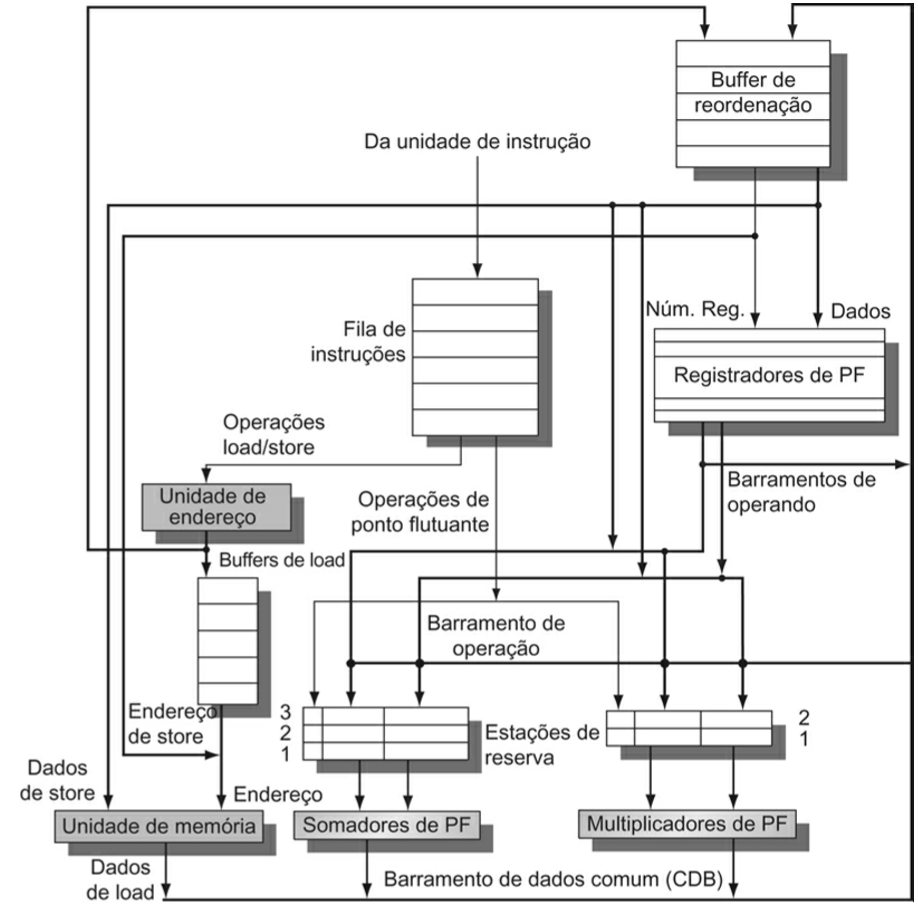
\includegraphics[width=.6\textwidth]{img/fig_tomasulo.png}
  \caption{Estrutura do Harware de Tomasulo. Fonte: Hennessy e Patterson (2019).}
  \label{fig_tomasulo}
\end{figure}


Considerando este esquema, o Algoritmo de Tomasulo oferece duas vantagens importantes, a primeira é a distribuição da lógica de detecção de riscos, através das Estações de Reservas (ES) distribuídas e do uso do Barramento Comum (CDB), a segunda, trata-se da eliminação de stalls para os riscos de WAW e WAR. Isso pode ocorrer através da renomeação de registradores das ES's e, também pelo processo de armazenar operando na estação de reserva quando estiverem disponíveis. Deste modo, o Algoritmo de Tomasulo torna-se uma ferramenta importante para execução das instruções distribuídas.

\subsubsection{Preditor de Desvio Baseados em Direção} \label{sec:secao_desvio}

Dentres o preditores, existem os estáticos e os dinâmicos. Os estáticos pressupõe que o desvio será independente do histórico de execução. Em contrapartida, os dinâmicos consideram o histórico.

Os Preditores de desvio baseado em direção, são estáticos e consideram a direção do desvio na memória para tomada de decisão. Neste caso, a comparação é entre o endereço de memória atual e o endereço do destino do desvio se faz necessária.

Neste trabalho serão consideradas duas versões de preditores estáticos: Desvios para endereços ``maiores'' \textit{TAKEN} (V1) e Devios para endereços ``maiores'' \textit{NOT TAKEN} (V2). Sendo que, o primeiro (V1), caso a comparação entre o endereço atual e o endereço de desvio indicar que o endereço de desvio é ``maior'', então o preditor ``pega(\textit{TAKEN})'' o desvio, caso contrário ``não pega (\textit{NOT TAKEN})'' o desvio. Da mesma maneira, o segundo (V2), caso a comparação entre o enderço atual e o endereço de desvio indicar que o endereço é ``maior'', então o preditor ``não pega (\textit{NOT TAKEN})'', caso contrário o preditor ``pega(\textit{TAKEN})''.


\section{Metodologia}

Para alcançar o propósito do trabalho, foram realizados ajustes no sistema TFSim \cite{lucas:2019}. Dentre eles de um botão ALL CYCLES, cálculo de algumas métricas de desempenho e a implementação de dois novos preditores estáticos descritas abaixo:

\begin{enumerate}
  \item Inclusão do botão \textit{ALL CYCLE} - realiza a execução de todos os ciclos de execução de trecho de Código, em MIPS.
  \item Métricas de Desempenho - contador de instruções, Instruções por ciclo (IPC), Milhões de Instruções por Segundo (MIPS) e tempo de execução de CPU; Disponível na parte não gráfica do sistema.
  \item Inclusão de dois novos Preditores estáticos \ref{sec:secao_desvio}:
        \begin{enumerate}
          \item Desvio para cima TAKEN (V1).
          \item Desvio para cima NOT TAKEN (V2).
        \end{enumerate}
  \item Inclusão do menu 'Trabalho' (Figura \ref{fig_menutfsim}) - para auxiliar na execução dos programas do trabalho, foi criado um menu, contento as opções de seleção de 3 novos programas e a opção de escolha dos desvios de predição desenvolvidos.
\end{enumerate}

\begin{figure}[h]
  \centering
  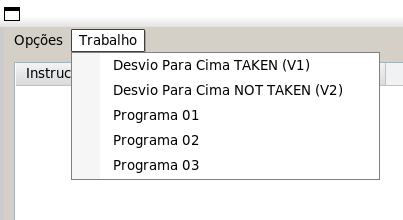
\includegraphics[width=.5\textwidth]{img/fig_menutfsim.png}
  \caption{Insterface do Novo Menu TFSim. Fonte: Elaboração Própria (2022).}
  \label{fig_menutfsim}
\end{figure}

Deste modo, na Figura \ref{fig_tfsim}, pode-se observar a interface do sistema que está organizada como segue:

\begin{enumerate}
  \item Fila de Instruções: mostra as instruções que estão sendo executadas durante a simulação, contendo informações como (despacho, execução, escrita e complemento);
  \item Estações de Reserva (RS): contém as informações de operandos, como nome da instrução, caso a instrução está ocupada ou não (\textit{Busy}), Op, $V_j$, $V_k$, $Q_j$, $Q_k$ e A;
  \item Banco de registradores: informa os valores de todos os registradores e qual estação de reserva (ou posição do ROB) está programado para escrever em cada registrador envolvido em uma determinada operação;
  \item Estrutura de Memória: Conjunto de valores das posições de memória;
  \item Buffer de Reordenação (ROB): informa quais instruções estão sendo executadas for a de ordem, apresentando seu destino e valor resultante (caso já tenham sido computadas);
  \item Área onde são exibidos os valores do ciclo de clock. Em um versão futura poderá ser trazida as métricas implementadas de modo não gráfica.
  \item Botões de controle de execução: \textit{START} – inicia a execução do primeiro código de sequência de códigos. \textit{NEXT CYCLE} – executa um ciclo por vez na sequência dada de códigos. \textit{ALL CYCLE} – executa todos os ciclos de uma determinada sequência, sem sair do programa e \textit{EXIT} – encerra a execução.
\end{enumerate}

\begin{figure}[h]
  \centering
  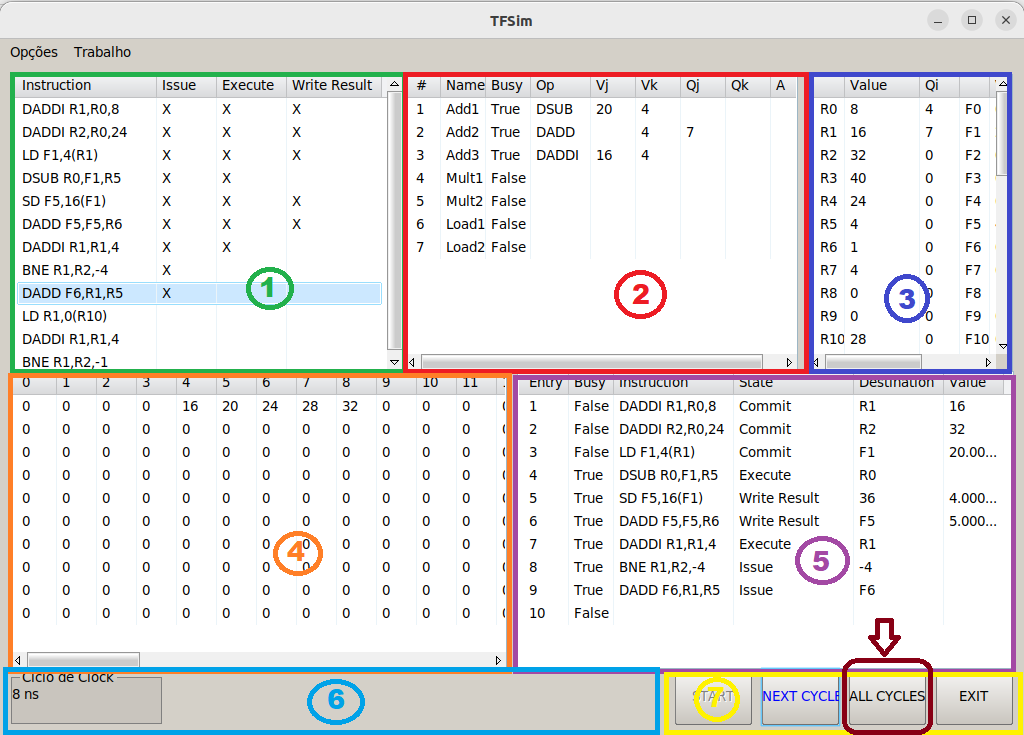
\includegraphics[width=.7\textwidth]{img/fig_tfsim.png}
  \caption{Insterface do TFSim. Fonte: Adaptado de dos Reis e Duenha (2019).}
  \label{fig_tfsim}
\end{figure}

\section{Análise e Discussão}

Para a análise, foi necessário a implementação de três programas para a realização dos experimentos. Desta forma, optou-se por definir programas pequenos de modo a viabilizar as execuções. Apesar do sistema (TFsim) já fornecer alguns exemplos de instruções, foram utilizados novos programas com inclução de algumas \textit{branchs} com interações que permitissem o \textbf{processamento superior a mil instruções}. Desta forma buscou-se a geração satisfatória de métricas. Além disso, considerou-se as seguintes latências:
DADD(2), DADDI(2), DSUB(2), DSUBI(2), DMUL(3), DDIV(3), MEM(1).

No programa 01, foi usado o \textit{branch} BNE com preponderância de desvio para baixo, incrementando o Registrador R1 até que ele fosse igual a R2. Durante o desenvolvimento, acrescentou-se no programa algumas instruções afim de ampliar o número de instruções no pipeline e também o leque de instruções utilizadas. No programa 2, buscou-se explorar laço dentro de laço, com uma instrução BNE externa, e um BEQ(com desvio para cima) e um BNE(com desvio para baixo) interno. E no programa 03, foi usada uma estrutura tripla de laços de repetição e, de forma análoga ao programa 02, adicionando um laço (do-while), com o desvio BNE (desvio para baixo) externo com 5 iterações.

Para cada programa, após o desenvolvimento e ajustes para o correto funcionamento, foram coletadas métricas de desempenho na utilização dos 2 novos preditores implementados: Desvio para cima TAKEN (V1) e Desvio para cima NOT TAKEN (V2). As métricas coletadas foram Número de Instruções (Comitadas) (NIC), Número de Instruções (NI) Executadas, Ciclos por Instrução (CPI), Tempo de CPU (CPU), Instruções por Segundo (MIPS) e Taxa de Acerto de Predição (TA).

Deste modo, a seguir na ... a compilação resultados da execução dos programas.


\begin{table}[ht]
  \caption{Estatísticas da Execução dos programas. Elaboração Própria (2022).}
  \begin{center}
    \label{tab_programas}
    \begin{tabular}{rcccccc}
      \hline
      \small{\textbf{Métricas}} & \multicolumn{2}{c}{\small{\textbf{Programa01}}} & \multicolumn{2}{c}{\small{\textbf{Programa02}}} & \multicolumn{2}{c}{\small{\textbf{Programa03}}}                                                                                                     \\
                                & V1                                              & V2                                              & V1                                              & V2                              & V1                             & V2                             \\
      \hline
      NI                        & \footnotesize{1529}                             & \footnotesize{1284}                             & \footnotesize{2596}                             & \footnotesize{1640}             & \footnotesize{3864}            & \footnotesize{2304}            \\
      NIC                       & \footnotesize{1275}                             & \footnotesize{1275}                             & \footnotesize{1412}                             & \footnotesize{1412}             & \footnotesize{2060}            & \footnotesize{2060}            \\
      CPI                       & \footnotesize{1.60392}                          & \footnotesize{1.01098}                          & \footnotesize{2.45963}                          & \footnotesize{1.49433}          & \footnotesize{1.88301}         & \footnotesize{1.12136}         \\
      CPU                       & \footnotesize{2.045x$10^{-6}$}                  & \footnotesize{1.289x$10^{-6}$}                  & \footnotesize{3.473x$10^{-6}$}                  & \footnotesize{2.11x$10^{-6}$}   & \footnotesize{3.879x$10^{-6}$} & \footnotesize{2.31x$10^{-6}$}  \\
      MIPS                      & \footnotesize{1.275x$10^{-12}$}                 & \footnotesize{1.275x$10^{-12}$}                 & \footnotesize{1.412x$10^{-12}$}                 & \footnotesize{1.412x$10^{-12}$} & \footnotesize{2.06x$10^{-12}$} & \footnotesize{2.06x$10^{-12}$} \\
      TA                        & \footnotesize{0.00393701}                       & \footnotesize{0.996078}                         & \footnotesize{0.358259}                         & \footnotesize{0.953125}         & \footnotesize{.378626}         & \footnotesize{0.949051}        \\
    \end{tabular}
  \end{center}
  \label{tab:multicol}
\end{table}

Como pode-se notar na Tabela \ref{tab_programas}, o programa 01, com a maioria dos ciclos para baixo (254), obteve, como esperado, melhor Taxa de Acerto com o Desvio para cima NOT TAKEN (V2),

\section{Conclusão}\label{sec:figs}

Compreender o processo de melhoria de hardware é essêncial na área de arquitetura de computadores. Uma estratégia para a análise de análise de métricas de desempenho é a utilização de simuladores. Neste trabalho, buscou-se simular a execução de 3 programas com intuito de coletar métricas de desempenho com utilização do \textbf{Algoritmo de Tomasulo} em conjunto com a  técnica de \textbf{Desvio de Predição Baseada em Direção} com apoio  do simulador TFSim \cite{lucas:2019}.

Para elaboração da pesquisa foi necessário realizar o embasamento teóricos das técnicas utilizadas, estudo do simulador, realização de implementação das novas funcionalidades em conjunto com pequenos ajustes na ferramenta, definição de métricas de desempenho, e por fim a elaboração e análise de 3 programas em MIPS. Dentre as funcionalidades desenvolvidas a inclusão do botão \textit{ALL CYCLE} que permite rodar o programa todo de uma vez, a inclusão de dois novos preditores  de Desvio para cima TAKEN (V1) e Desvio para baixo NOT TAKEN (V2), e, a inclusão de métricas na área não gráfica do programa.

Deste modo, buscou-se no desenvolvimento dos programas explorar os desvios para cima e para baixo de modo a garantir uma análise adequada do desempenho dos preditores. Sendo que este desempenho está relacionado a características dos programas.

..... Aqui resumo da nossa análise...

Assim sendo, cabe sugerir, para pesquisas futuras, a inclusão na ferramenta TFSim de um botão     ``Pause/Stop'', para verificação dos valores no meio da execução. Um botão ``Reiniciar'' para que não seja necessário sair da aplicação a cada execução. E por fim, inclusão de métricas na interface gráfica.

\bibliographystyle{sbc}
\bibliography{sbc-template}

\end{document}
